\newpage

%%%%%%%%%%%%%%%%%%%%%%%%%%%%%%%%%%%%%%%%%%%%%%%%%%%%%%%%%%%%%%%%%%%%%%%%%%%%%%%%%%%%%%%
%%%%%%%%%%%%%%%%%%%%%%%%%%%%%%%%%%%%%%%%%%%%%%%%%%%%%%%%%%%%%%%%%%%%%%%%%%%%%%%%%%%%%%%
%%%%%%%%%%%%%%%%%%%%%%%%%%%%%%%%%%%%%%%%%%%%%%%%%%%%%%%%%%%%%%%%%%%%%%%%%%%%%%%%%%%%%%%
\section{Regressão logística e SE com classificador $f_{\VECTOR{c}}(\VECTOR{x}):~\mathbb{R}^{N} \rightarrow \mathbb{R}$}
\label{sec:theo:reglogrnr1:1}

\index{Regressão!Logística $f_{\VECTOR{c}}(\VECTOR{x}):~\mathbb{R}^{N} \rightarrow \mathbb{R}$}



\begin{theorem}[Classificação de dados em $\mathbb{R}^{N}$:]\label{theo:reglogrnr1:1}
~\\
\noindent
\begin{minipage}{0.45\textwidth}
\centering
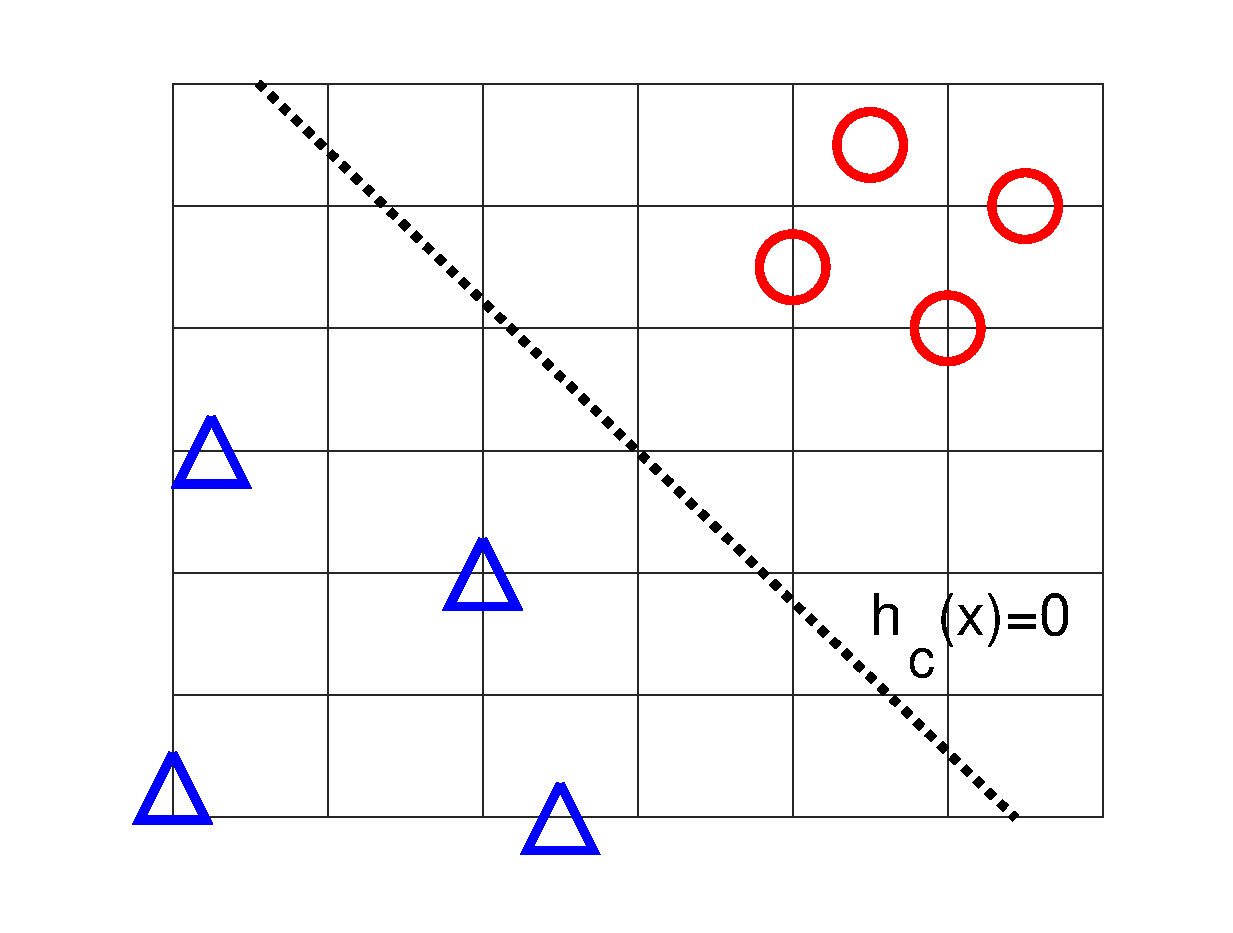
\includegraphics[width=0.95\linewidth]{chapters/classificacao/mfiles/reglogrnr1/reglogrnr1.eps} 
\end{minipage}
\begin{minipage}{0.55\textwidth}
Dados, um conjunto de $L$ pontos
$\VECTOR{x}_l$ $\in \mathbb{R}^{N}$, $1\leq l \leq L$,
repartidos em dois grupos etiquetados com os símbolos $\bigtriangleup$ e $\bigcirc$,
separáveis por um hiperplano  em $\mathbb{R}^{N}$.
Se desejamos criar um classificador mediante 
a função  $f_{\VECTOR{c}}:\mathbb{R}^{N} \rightarrow \mathbb{R}$,
com domínio $\VECTOR{x} \in \mathbb{R}^{N}$, contradomínio $y \in \mathbb{R}$ e 
parâmetros agrupados no vetor $\VECTOR{c}=[c_1$ $c_2$ $...$ $c_{N+1}]^{\transpose}\in \mathbb{R}^{N+1}$,
como definido na Eq. (\ref{eq:reglogrnr1:1}),
\begin{equation}\label{eq:reglogrnr1:1}
y\equiv f_{\VECTOR{c}}(\VECTOR{x})= \frac{1}{1+e^{-h_{\VECTOR{c}}(\VECTOR{x})}},
\quad h_{\VECTOR{c}}(\VECTOR{x})=[1\quad \VECTOR{x}^{\transpose}] \VECTOR{c},
\end{equation}
ou seu equivalente: $logit(y)=h_{\VECTOR{c}}(\VECTOR{x})$.
\end{minipage}

Podemos atribuir a cada ponto $\VECTOR{x}_l$ uma etiqueta $y_l\in \{A,1-A\}$, 
$A$ para $\bigtriangleup$ e  $1-A$ para $\bigcirc$,
onde $0<A\ll 0.5$ é escolhido por nós,
e afirmar que o vetor $\VECTOR{c}= \VECTOR{\hat{c}}$,
que minimiza o erro quadrático $e(\VECTOR{c})$,
\begin{equation}\label{eq:reglogrnr1:1e}
e(\VECTOR{c}) =  \sum_{l=1}^{L} w_l||h_{\VECTOR{c}}(\VECTOR{x}_l)-logit(y_l)||^2,
\end{equation}
pode ser achado\footnote{A demostração pode ser vista na Prova \ref{proof:theo:reglogrnr1}.}  
mediante a Eq. (\ref{eq:reglogrnr1:2}), 
sendo que é considerado que os erros de cada amostra $\VECTOR{x}_l$ em $e(\VECTOR{c})$ são ponderados 
mediante os pesos $w_l \in \mathbb{R}_+$,
\begin{equation}\label{eq:reglogrnr1:2}
\VECTOR{\hat{c}} =  \left[ \MATRIX{A}^{\transpose} \MATRIX{W}\MATRIX{A}\right]^{-1} \MATRIX{A}^{\transpose} \MATRIX{W}\VECTOR{z},
\quad
\MATRIX{A}=
\begin{bmatrix}
1 & \VECTOR{x}_1^{\transpose}\\
1 & \VECTOR{x}_2^{\transpose}\\
\vdots & \vdots\\
1 & \VECTOR{x}_l^{\transpose}\\
\vdots & \vdots\\
1 & \VECTOR{x}_L^{\transpose}\\ 
\end{bmatrix},
\quad
\VECTOR{z}=
\begin{bmatrix}
logit(y_1)  \\
logit(y_2)  \\
\vdots  \\
logit(y_l)  \\
\vdots \\
logit(y_L) \\
\end{bmatrix},
\quad
\MATRIX{W}=\funcdiag \left(
\begin{bmatrix}
w_1 \\
w_2 \\
\vdots  \\
w_l \\
\vdots \\
w_L \\
\end{bmatrix} \right).
\end{equation}
%e agrupados na matriz  $\MATRIX{W}=\funcdiag \left( \left[w_1,~ w_2,~ ...,~ w_L \right]^{\transpose} \right) $.
\end{theorem}

\begin{tcbattention}
\begin{itemize}
\item Dado que a função de classificação $f_{\VECTOR{c}}(\VECTOR{x})$ vai entre $0$ e $1$,
podemos reinterpretar este valor como se fosse uma probabilidade;
neste caso, $f_{\VECTOR{c}}(\VECTOR{x}_l)$ representa, $P(y_l=\bigcirc|\VECTOR{x}_l)$, 
a probabilidade de que $y_l=\bigcirc$ dado que tivemos como entrada o ponto $\VECTOR{x}_l$.
\item O limiar de classificação na função $f_{\VECTOR{c}}(\VECTOR{x})$ está no hiperplano $h_{\VECTOR{c}}(\VECTOR{x})=0$,
provocando nestos pontos um $f_{\VECTOR{c}}(\VECTOR{x})=0.5$.
\end{itemize}
\end{tcbattention}



%%%%%%%%%%%%%%%%%%%%%%%%%%%%%%%%%%%%%%%%%%%%%%%%%%%%%%%%%%%%%%%%%%%%%%%%%%%%%%%%
\subsection{Exemplos de classificação com uma função
$f_{\VECTOR{c}}(\VECTOR{x}):~\mathbb{R}^N \rightarrow \mathbb{R}$ }

\begin{example}\label{ex:theo:reglogrnr1}
Conhecidas as $L=10$ amostras $\VECTOR{x}_l$ e seus respetivos grupos indicados pelos símbolos $\bigtriangleup$ e $\bigcirc$, 
mostrados na Tabela \ref{table:theo:reglogrnr1:xn},
achar o classificador $f_{\VECTOR{c}}(\VECTOR{x})$, 
que gere o menor erro $e(\VECTOR{c}) =  \sum_{l=1}^{L} ||h_{\VECTOR{c}}(\VECTOR{x}_l)-logit(y_l)||^2$.
\end{example}


\begin{table}[h!]
\centering
\begin{tabular}{|c||c|c|c|c|c||c|c|c|c|c||} 
 \hline
$l$            & 1 & 2 & 3 & 4 & 5 & 6 & 7 & 8 & 9 & 10 \\ \hline \hline
$\VECTOR{x}_l$ & 1 & 3 & 1 & 2 & 1 & 4 & 5 & 6 & 3 & 2 \\ 
~              & 1 & 1 & 4 & 2 & 2 & 4 & 3 & 2 & 5 & 6 \\ \hline
$\VECTOR{y}_l$ & $\bigtriangleup$ & $\bigtriangleup$ & $\bigtriangleup$ & $\bigtriangleup$ & $\bigtriangleup$ 
      & $\bigcirc$ & $\bigcirc$ & $\bigcirc$ & $\bigcirc$ & $\bigcirc$\\ \hline
\end{tabular}
\caption{Pontos $\VECTOR{x}_l$.}
\label{table:theo:reglogrnr1:xn}
\end{table}


\begin{SolutionT}[Relativa ao Exemplo \ref{ex:theo:reglogrnr1}:]\label{sol:theo:reglogrnr1:s1}
Para obter o vetor de parâmetros $\VECTOR{c}=\VECTOR{\hat{c}}$ da função $f_{\VECTOR{c}}(\VECTOR{x})$, 
que gere o menor erro $e(\VECTOR{c}) =  \sum_{l=1}^{L} ||h_{\VECTOR{c}}(\VECTOR{x}_l)-logit(y_l)||^2$
com os $L=10$ dados $\VECTOR{x}_l$ da Tabela \ref{table:theo:reglogrnr1:xn},
usamos a Eq. (\ref{eq:reglogrnr1:2}) onde escolhemos $w_l=1$ e valores $y_l \in \{0.1,~ 0.9\}$,
$0.1$ para $\bigtriangleup$ e $0.9$ para $\bigcirc$,
obtendo um vetor $\VECTOR{\hat{c}}=[-5.21014\quad 0.95532\quad 0.84509]^{\transpose}$.
Assim, podemos representar a função $\left.f_{\VECTOR{c}}(\VECTOR{x})\right|_{\VECTOR{c}=\VECTOR{\hat{c}}}$
 que classifica os dados $\VECTOR{x}_l$, 
como é mostrado na Figura \ref{fig:theo:reglogrnr1:xn:s1},
\begin{equation}
f_{\VECTOR{\hat{c}}}(\VECTOR{x})= \frac{1}{1+e^{-(-5.21014  +0.95532 x_1+ 0.84509 x_2)}}.
\end{equation}
É interessante ressaltar que a pendente é pequena e a classificação é pouco definida,
com limiares de classificação no hiperplano $-5.21014  +0.95532 x_1+ 0.84509 x_2=0$.
\end{SolutionT}

\begin{figure}[!h]
    \begin{subfigure}[b]{0.45\textwidth}
        \centering
        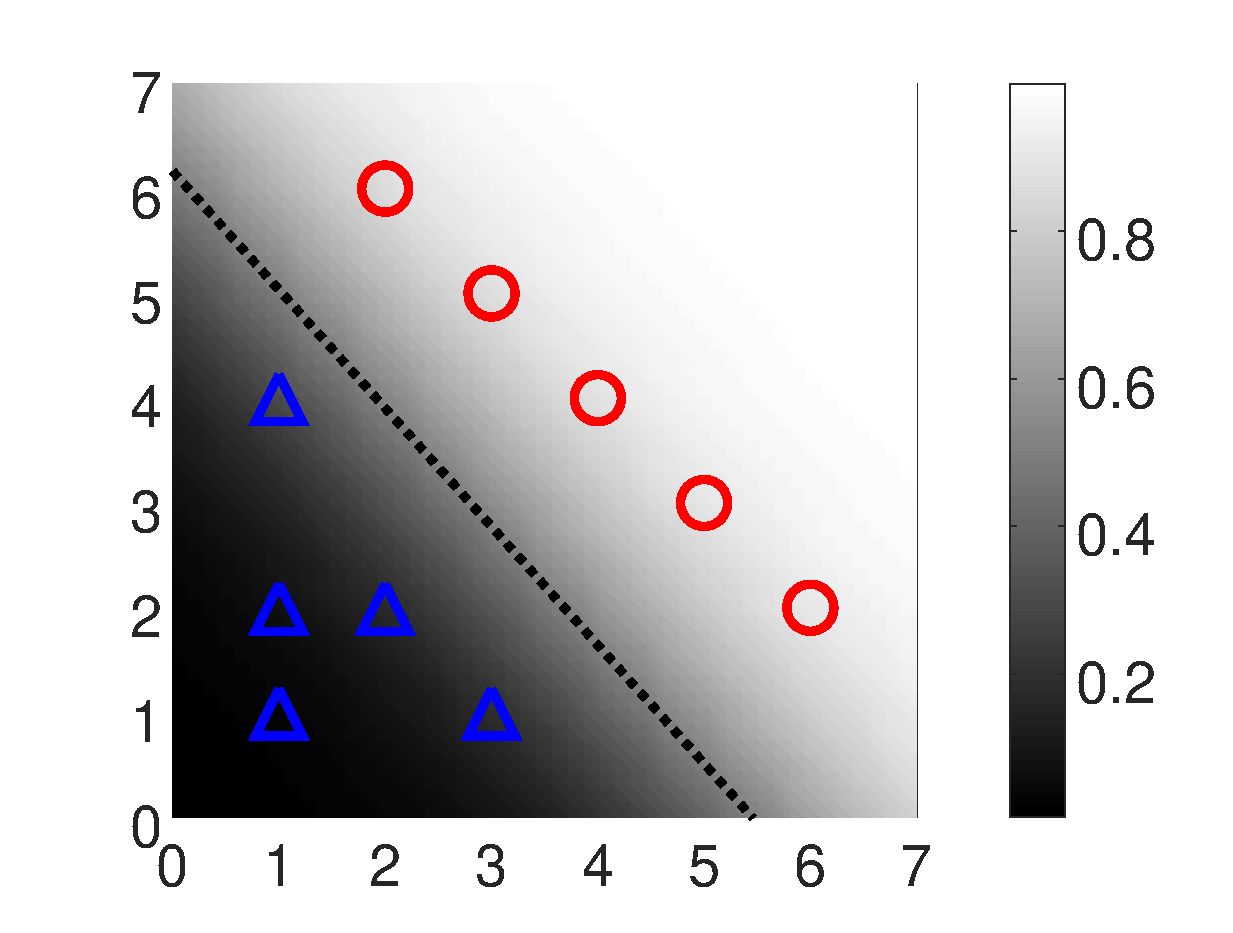
\includegraphics[width=\textwidth]{chapters/classificacao/mfiles/reglogrnr1/ex1s1-reglogrnr1.eps}
        \caption{Gráfico da classificação usando $y_l \in \{0.1,~ 0.9\}$.}
        \label{fig:theo:reglogrnr1:xn:s1}
    \end{subfigure}
    \hfill
    \begin{subfigure}[b]{0.45\textwidth}
        \centering
        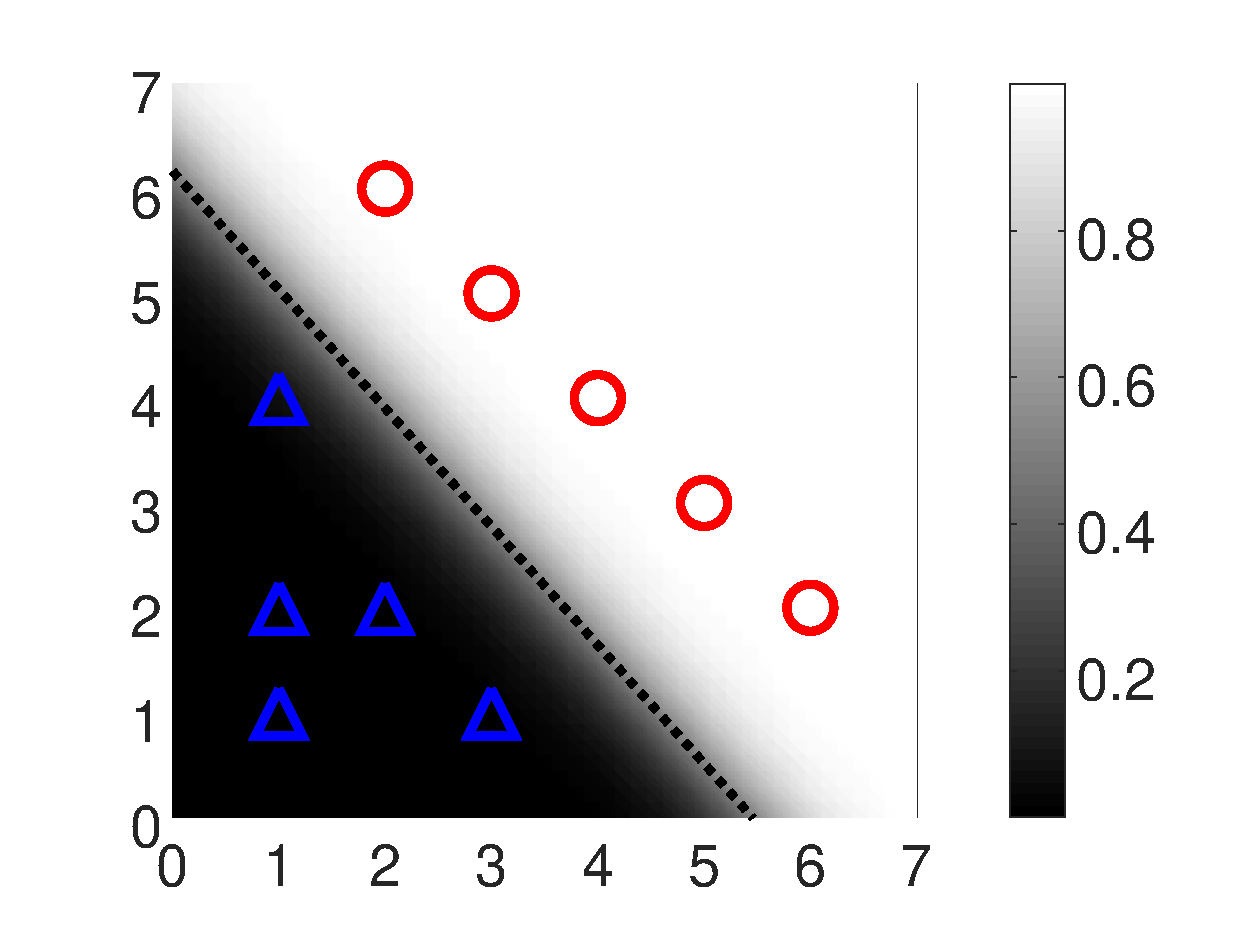
\includegraphics[width=\textwidth]{chapters/classificacao/mfiles/reglogrnr1/ex1s2-reglogrnr1.eps}
        \caption{Gráfico da classificação usando $y_l \in \{0.001,~ 0.999\}$.}
        \label{fig:theo:reglogrnr1:xn:s2}
    \end{subfigure}
    \caption{Classificação usando a função $f_{\VECTOR{\hat{c}}}(\VECTOR{x})$.}
    \label{fig:theo:reglogrnr1:xn}
\end{figure}


\begin{SolutionT}[Relativa ao Exemplo \ref{ex:theo:reglogrnr1}:]\label{sol:theo:reglogrnr1:s2}
Para obter o vetor de parâmetros $\VECTOR{c}=\VECTOR{\hat{c}}$ da função $f_{\VECTOR{c}}(\VECTOR{x})$, 
que gere o menor erro $e(\VECTOR{c}) =  \sum_{l=1}^{L} ||h_{\VECTOR{c}}(\VECTOR{x}_l)-logit(y_l)||^2$
com os $L=10$ dados $\VECTOR{x}_l$ da Tabela \ref{table:theo:reglogrnr1:xn},
usamos a Eq. (\ref{eq:reglogrnr1:2}) onde escolhemos $w_l=1$ e valores $y_l \in \{0.001,~ 0.999\}$,
$0.001$ para $\bigtriangleup$ e $0.999$ para $\bigcirc$,
obtendo um vetor $\VECTOR{\hat{c}}=[-16.3776\quad 3.0029\quad 2.6564]^{\transpose}$. 
Assim, podemos representar a função $\left.f_{\VECTOR{c}}(\VECTOR{x})\right|_{\VECTOR{c}=\VECTOR{\hat{c}}}$ 
que classifica os dados $\VECTOR{x}_l$, 
como é mostrado na Figura \ref{fig:theo:reglogrnr1:xn:s2} e na Eq. (\ref{eq:theo:reglogrnr1:xn:s2}),
\begin{equation}\label{eq:theo:reglogrnr1:xn:s2}
f_{\VECTOR{\hat{c}}}(\VECTOR{x})= \frac{1}{1+e^{-(-16.3776+3.0029 x_1 +2.6564 x_2)}}.
\end{equation}
É interessante ressaltar que a pendente é abrupta para cada grupo com uma classificação bem definida,
e limiares de classificação no hiperplano $-16.3776+3.0029 x_1 +2.6564 x_2=0$.
\end{SolutionT}
